\section{Aufbau}
\label{sec:Aufbau}

\begin{figure}
 \centering
 \caption{Der schematische Aufbau des verwendeten Augenmodells.\cite{US1}}
 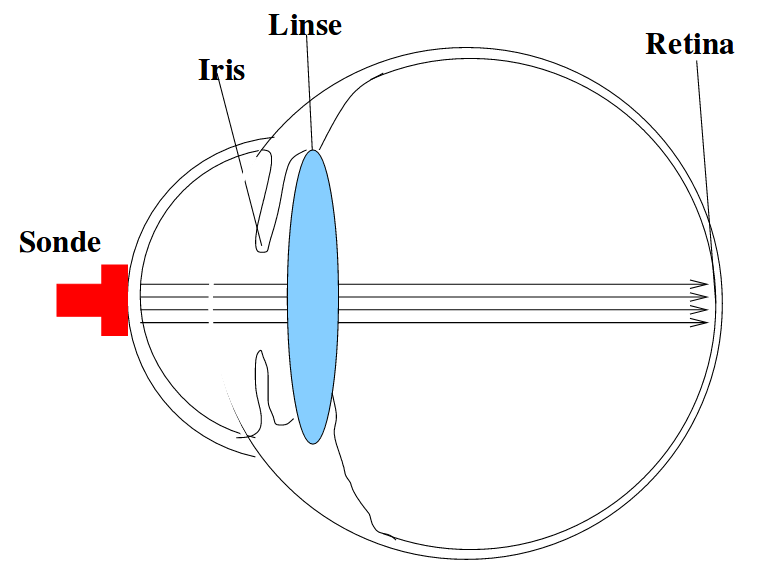
\includegraphics[width=\linewidth-170pt,height=\textheight-170pt,keepaspectratio]{content/AUGE.png}
 \label{fig:auge}
\end{figure}

Der Versuchsaufbau besteht aus 2 Messsonden, welche mit $\SI{2}{\mega\hertz}$
betrieben werden, einem Ultraschallechoskop und einem Computer zur Aufnahme der Daten.
Am Ultraschallechoskop lässt sich einstellen ob die jeweilige Sonde als Sender,
Empfänger oder beides fungieren soll. Zusätzlich kann eine Verstärkung der
auftretenden Signale eingestellt werden. Dies geschieht sowohl über einen zeitlich konstanten Verstärkungsfaktor,
welcher über die Einstellung Gain justiert wird, als auch über eine zeitlich
veränderlichen, den sogennanten  TCG. Letzterer beschreibt eine zeitlich linear ansteigende Verstärkung
und kann über die Parameter $Threshold$, $Wide$, $Slope$ und $Start$
modifiziert werden. Die gemessenen Signale werden mithilfe der
Software AScan ausgewertet. Ein Ascan lässt sich über den Menüpunkt Ascan starten. Im oberen
Graphen werden die auftretenden Peaks, im unteren der zugehörige TCG Wert
dargestellt. Mithilfe von einblendbaren Cursern können die Peaks präziser vermessen
werden. Über die Funktion FFT wird zusätzlich das Spektrum sowie ihr zugehöriges
Cepstrum angezeigt. Für die dafür benötigten Berechnungen wird nur der
Graphenabschnitt verwendet der sich zwischen zwei Cursern befindet.
Für den letzten Versuchteil wird zusätzlich ein Augenmodell nach Abb. \ref{fig:auge} mit Maßstab 3:1 verwendet.
